\documentclass[fontsize=10pt,a4paper]{scrbook}
\usepackage{pdfpages}
\usepackage{book/styles/myusepackages}
\usepackage{book/styles/mypythonstyle}
\usepackage{book/styles/myMCquestions}
\usepackage{book/styles/myframedenv}
%If graphics is listed before,some problems arise
\usepackage{graphicx}

\usepackage[spanish]{babel}
\usepackage[spanish,verbose]{layout}
%\hypersetup{pdflang={es-ES}}

%\newcommand{\academicyear}{2023-2024}


%%%%%%
\usepackage{parskip}
\usepackage{amsmath,amssymb,amsfonts,latexsym}
\usepackage{xparse}
\usepackage{tcolorbox}        
\tcbuselibrary{skins,breakable} 

%%%%%%%EXERCISES

\usepackage{etoolbox}
\usepackage{tcolorbox}

% Define boolean variable to check if overlay has been drawn
\newif\ifMyExerciseBoxOverlayDrawn
\MyExerciseBoxOverlayDrawnfalse

\definecolor{color2}{RGB}{117,184,68}
\colorlet{color1}{green!2!white}

\newcounter{myexercise}[chapter]
\renewcommand{\themyexercise}{\thechapter.\arabic{myexercise}}

\newtcolorbox{myexercisebox}{%
    enhanced,
    colback=color1,
    colframe=color2,
    arc=0mm,
    boxrule=0pt,
    top=10mm,
    bottom=2mm,
    left=0mm,
    right=0mm,
    enlarge top by=0mm,
    enlarge top at break by=0mm,
    pad at break=0mm,
    fontupper=\normalsize,
    breakable,   % allow page breaks
    overlay ={
        \begin{tcbclipinterior}
        \pgfmathsetmacro{\OverlayDrawn}{0}
        \ifcsname myexerciseboxoverlaydrawn\themyexercise\endcsname
          \pgfmathsetmacro{\OverlayDrawn}{1}
        \else
          \node[rectangle, minimum width=1cm, minimum height=0.5cm, top color=color2, bottom color=color2, inner sep=1mm,anchor=west,font=\normalsize, text=white, yshift=-5mm] at ([xshift=0mm]frame.north west)%
          {\textbf{\themyexercise}};
          \global\expandafter\let\csname myexerciseboxoverlaydrawn\themyexercise\endcsname\relax
        \fi
        \end{tcbclipinterior}
    }
}

\newenvironment{ejercicio}{%
    \refstepcounter{myexercise}%
    \bigskip%
    \begin{myexercisebox}%
    \noindent\ignorespaces%
    }{%
    \end{myexercisebox}%
    %\medskip%
    }

%%%%%%%EXERCISES

\usepackage{scrindex}
\makeindex

\begin{document}



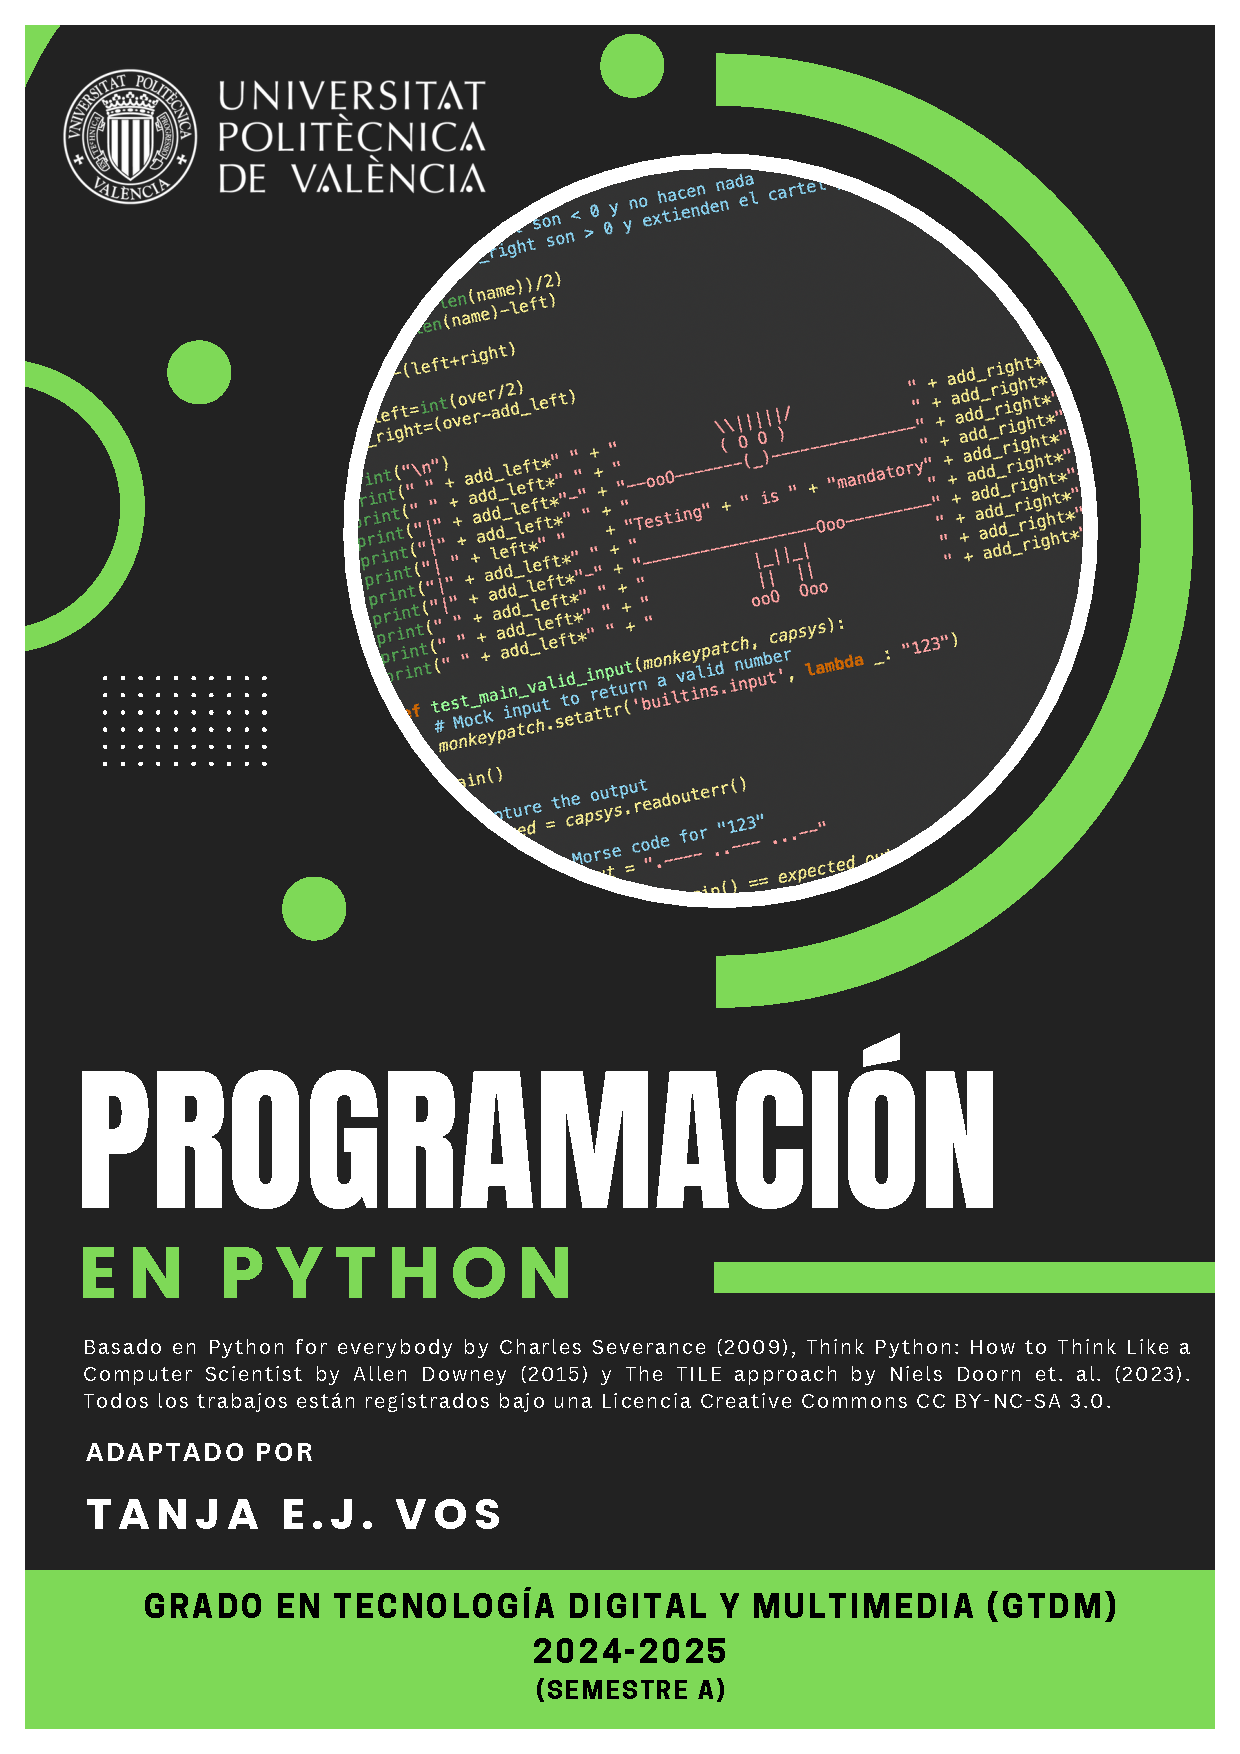
\includepdf[fitpaper]{voorkant2024.pdf}
\newpage
\thispagestyle{empty}
\vspace*{2.0cm}
\newpage
%%%%%%%%%%%%%%%%%%%%%%%%%%%%%%%%%%%%%%%%%%%%%%%%
%%%%%%%%%%%% TITLE
%\begin{center}
%\begin{Huge}
%\textbf{Programación en Python}

%\vspace*{0.5cm}

%\academicyear{}\\
%\end{Huge}
%\end{center}

%\begin{footnotesize}
%\noindent El contenido de este libro esta basada en material de diferente libros open source: \textit{Python for everybody}, Copyright 2009 - Charles Severance, and  \textit{Think Python: How to Think Like a Computer Scientist}, Copyright 2015 - Allen Downey.Ambos trabajos están registrados bajo una Licencia Creative Commons Attribution-NonCommercial-ShareAlike 3.0 Unported License. Este licencia está disponible en \url{http://creativecommons.org/licenses/by-nc-sa/3.0/}.
%\end{footnotesize}

\begin{center}
%\textbf{Adaptado y extendido por Tanja E. J. Vos}

%\vspace*{0.2cm}

%\Large{\textbf{Universidad Politécnica de Valencia}}
%\vspace*{2.0cm}
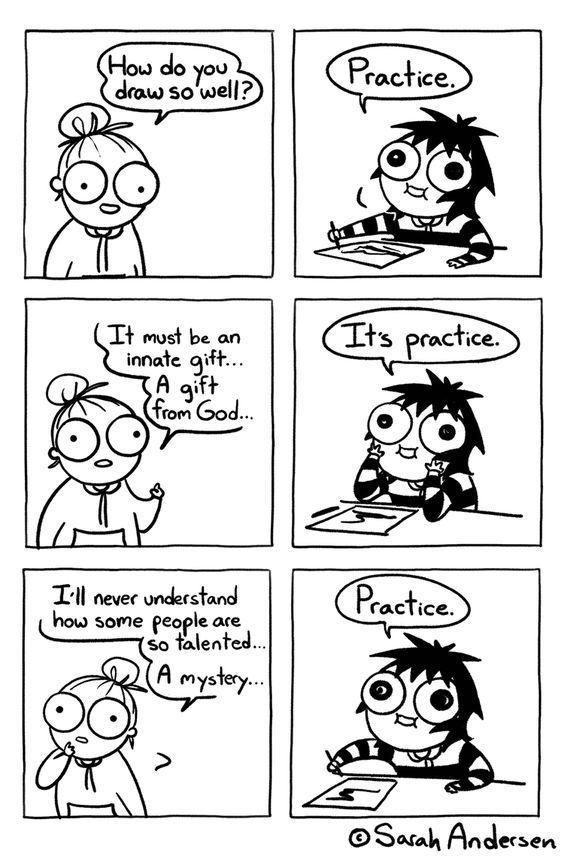
\includegraphics[width=\textwidth]{book/practicarPIC.jpeg}
\end{center}
\newpage
\vspace*{2.0cm}
\newpage


%%%%%%%%%%%%%%%%%%%END TITLE%%%%%%%%%%%%%%%%%%%%%
\dominitoc% Initialization
\tableofcontents


\chapter*{Prólogo}
\addcontentsline{toc}{chapter}{Prólogo}


¡Bienvenido a este libro de Python que te acompañará en el tema de programación durante el primer semestre de tus estudios universitarios!

Este libro se inspira en dos obras de código abierto:\textit{Python for Everybody} de Charles Severance \cite{severance2016python} y \textit{Think Python: How to Think Like a Computer Scientist} de Allen Downey \cite{downey2016thinkpython}. Estos libros han compartido su conocimiento bajo licencias de Creative Commons, formando la base del contenido de este libro.

La motivación para crear este libro surge de la necesidad de comprender sólidamente las pruebas (o el «testing») en la educación de programación. Creemos que las pruebas son una habilidad esencial en el mundo de la programación, pero sorprendentemente, este aspecto crucial a menudo se pasa por alto en los libros de programación para principiantes. Con el libro que tienes en tus manos, buscamos cambiar eso.

Integrar el «testing» en un curso de programación para principiantes no es fácil. Es por eso que utilizamos el innovador enfoque TILE \cite{10132188} «Test Informed Learning with Examples» o el Aprendizaje Informado por Pruebas con Ejemplos. El enfoque TILE se centra en integrar las pruebas de software en tu experiencia de programación introductoria de manera efectiva y placentera. TILE fue desarrollado con el generoso apoyo y financiamiento del proyecto Erasmus+ QPeD (número de contrato 2020-1-NL01-KA203-064626) y del proyecto ENACTEST (número de proyecto 101055874).

Con TILE, las pruebas se convierten en una parte integral de tu trayecto de programación desde el principio. Creemos firmemente que las pruebas no deben ser una idea secundaria, sino un aspecto esencial de tu proceso de codificación. Por eso te presentamos las pruebas desde el primer programa de ejemplo que encuentres.

Nuestro objetivo es dotarte del conocimiento y las habilidades para que te conviertas en un programador Python competente, armado con el poder de las pruebas para crear programas de alta calidad.

Así que, mientras te sumerges en el emocionante mundo de Python, recuerda que este libro está aquí para guiarte paso a paso en el dominio tanto de la programación como de las pruebas. Juntos, embarquémonos en este viaje mientras exploramos las maravillas de Python y el arte de las pruebas de software.

¡Feliz aprendizaje!

Tanja Vos
(tvos@dsic.upv.es)

%\newpage

\bibliography{biblio}
\bibliographystyle{unsrt}

\chapter{Introducción}
\minitoc% Creating an actual minitoc
\subimport{Spanish/01_Introduccion}{tema1}
\subimport{Spanish/01_Introduccion}{tema1_ejercicios}

\chapter{Valores, variables, tipos, operadores y expresiones.}
\minitoc% Creating an actual minitoc
\subimport{Spanish/02_Valores_Variables_Tipos_etc}{tema2}
\subimport{Spanish/02_Valores_Variables_Tipos_etc}{tema2_ejercicios}
\subimport{Spanish/02_Valores_Variables_Tipos_etc}{tema2_ejercicios_tipo_test}

\chapter{Conditional statements}
\minitoc% Creating an actual minitoc
\subimport{Spanish/03_Conditionals_if_elif_else}{tema3}
\subimport{Spanish/03_Conditionals_if_elif_else}{tema3_ejercicios}
\subimport{Spanish/03_Conditionals_if_elif_else}{tema3_ejercicios_tipo_test}

\chapter{Bucles}
\minitoc% Creating an actual minitoc
\subimport{Spanish/04_Bucles}{tema4}
\subimport{Spanish/04_Bucles}{tema4_ejercicios}
\subimport{Spanish/04_Bucles}{tema4_ejercicios_tipo_test}

\chapter{Funciones}
\minitoc% Creating an actual minitoc
\subimport{Spanish/05_Funciones}{tema5}
\subimport{Spanish/05_Funciones}{tema5_ejercicios}
\subimport{Spanish/05_Funciones}{tema5_ejercicios_tipo_test}
\subimport{Spanish/05_Funciones}{tema5_proyecto}

\chapter{Ficheros}
\minitoc% Creating an actual minitoc
\subimport{Spanish/06_Ficheros}{tema6}
\subimport{Spanish/06_Ficheros}{tema6_ejercicios}
\subimport{Spanish/06_Ficheros}{tema6_ejercicios_tipo_test}

\addcontentsline{toc}{chapter}{Índice}
\printindex[default]
\newpage
\vspace*{2.0cm}
\thispagestyle{empty}


\includepdf[fitpaper]{achterkant2024.pdf}




\end{document}

\chapter{Más sobre listas: mutabilidad y comprensiones}
\minitoc% Creating an actual minitoc
\subimport{Spanish/07_Listas}{tema7}
\subimport{Spanish/07_Listas}{tema7_ejercicios}

\chapter{Diccionarios}
\minitoc% Creating an actual minitoc
\subimport{Spanish/08_Diccionarios}{tema8}
\subimport{Spanish/08_Diccionarios}{tema8_ejercicios}

\chapter{Tuplas}
\minitoc% Creating an actual minitoc
\subimport{Spanish/09_Tuplas}{tema9}
\subimport{Spanish/09_Tuplas}{tema9_ejercicios}

\chapter{Conjuntos}
\minitoc% Creating an actual minitoc
\subimport{Spanish/10_Conjuntos}{tema10}
\subimport{Spanish/10_Conjuntos}{tema10_ejercicios}




